\documentclass[a4paper,12pt,twoside]{article}
\usepackage[left=1in,right=1in,top=1in,bottom=1in]{geometry}

\usepackage{xeCJK}
\setCJKmainfont{Songti TC}
\setCJKfamilyfont{kai}{Songti TC}
\newcommand{\kai}{\CJKfamily{kai}} % 用 \kai{使用楷書}

\usepackage{lmodern}
\usepackage{titling}
\usepackage{titlesec}
\usepackage{graphicx}
\usepackage{float}
\usepackage{amsmath, amsthm, amssymb, amsfonts, mathrsfs}
\usepackage{upgreek} % 直立的希臘字母

\usepackage[shortlabels]{enumitem}
\usepackage{setspace}
\renewcommand{\baselinestretch}{1.5}
\usepackage[colorlinks]{hyperref}
\usepackage{fancyvrb}
\usepackage{fancyhdr}
\usepackage{multicol}
\usepackage{caption}
\usepackage{subcaption}
\usepackage{listings}
\usepackage{bm}
\usepackage{bbm} % for \mathbbm{1} (indicator function)
\usepackage{centernot}
\usepackage{mdframed}
\usepackage{xltabular}
\usepackage{tcolorbox}
\tcbuselibrary{skins, breakable}
\usepackage{tikz}
\usetikzlibrary{patterns, arrows.meta, positioning, calc, decorations.pathmorphing, decorations.pathreplacing, decorations.markings, decorations.shapes, angles, quotes, 3d, matrix}
\usepackage[nameinlink, capitalise]{cleveref}
\usepackage{diagbox}
\usepackage{booktabs}
\usepackage{multirow,array}
\usepackage{tabularx}
\usepackage{mathtools}
\usepackage{indentfirst} % 首段 indent
\setlength{\parindent}{2em}
\usepackage{cancel} % 數學式子畫線槓掉
\newcommand\mcancel[2][red]{\setbox0=\hbox{$#2$}%
\rlap{\raisebox{.45\ht0}{\textcolor{#1}{\rule{\wd0}{1pt}}}}#2}
\setcounter{MaxMatrixCols}{20}
\usepackage{datetime2}
\usepackage{paracol}

\makeatletter
\def\tiangan#1{\expandafter\@tiangan\csname c@#1\endcsname}
\def\@tiangan#1{%
  \ifcase#1\or (甲)\or (乙)\or (丙)\or (丁)\or (戊)\or (己)\or (庚)\or (辛)\or (壬)\or (癸)\else(?)\fi
}
\AddEnumerateCounter{\tiangan}{\@tiangan}{(甲)}
\makeatother

% 支援 \wideparen 圓弧記號（若未載入 yhmath，可用此巨集穩定渲染）
\providecommand{\wideparen}[1]{\overset{\frown}{#1}}
\providecommand{\redtext}[1]{{\color{red} #1}}
\providecommand{\bluetext}[1]{{\color{blue} #1}}

\AtBeginDocument{%
 \setlength{\abovedisplayskip}{6pt}
 \setlength{\belowdisplayskip}{6pt}
 \setlength{\abovedisplayshortskip}{4pt}
 \setlength{\belowdisplayshortskip}{4pt}
}

\definecolor{codegreen}{rgb}{0,0.6,0}
\definecolor{codegray}{rgb}{0.5,0.5,0.5}
\definecolor{codepurple}{rgb}{0.58,0,0.82}
\definecolor{backcolour}{rgb}{0.95,0.95,0.92}

\lstdefinestyle{mystyle}{
 backgroundcolor=\color{backcolour},
 commentstyle=\color{codegreen},
 keywordstyle=\color{magenta},
 numberstyle=\tiny\color{codegray},
 stringstyle=\color{codepurple},
 basicstyle=\ttfamily\footnotesize,
 breakatwhitespace=false,
 breaklines=true,
 captionpos=b,
 keepspaces=true,
 numbers=left,
 numbersep=5pt,
 showspaces=false,
 showstringspaces=false,
 showtabs=false,
 tabsize=2
}
\lstset{style=mystyle}

\hypersetup{citecolor=blue, linkcolor=blue, urlcolor=blue}

\DeclareMathOperator{\supp}{supp}
\DeclareMathOperator{\skewness}{Skewness}
\DeclareMathOperator{\DU}{D-U}
\DeclareMathOperator{\CU}{C-U}
\DeclareMathOperator{\Geo}{Geo}
\DeclareMathOperator{\Pois}{Pois}
\DeclareMathOperator{\Gam}{Gam}
\DeclareMathOperator{\LN}{LogN}
\DeclareMathOperator{\cov}{Cov}
\DeclareMathOperator*{\argmax}{arg\,max}
\DeclareMathOperator*{\argmin}{arg\,min}
\DeclareMathOperator{\re}{Re}
\DeclareMathOperator{\im}{Im}

\newcommand{\N}{\mathbb{N}}
\newcommand{\Z}{\mathbb{Z}}
\newcommand{\Q}{\mathbb{Q}}
\newcommand{\R}{\mathbb{R}}
\newcommand{\C}{\mathbb{C}}
\newcommand{\G}{\mathcal{G}}
\newcommand{\mP}{\mathbb{P}}
\newcommand{\F}{\mathcal{F}}
\newcommand{\B}{\mathcal{B}}
\newcommand{\1}{\mathbbm{1}}
\newcommand{\Poi}{\text{Poi}}
\newcommand{\Var}{\text{Var}}
\newcommand{\as}{\text{a.s.}}
\newcommand{\vect}[1]{\boldsymbol{\mathbf{#1}}}
\newcommand{\paren}[1]{\left({#1}\right)}
\newcommand{\brk}[1]{\left[{#1}\right]}
\newcommand{\curl}[1]{\left\{{#1}\right\}}
\providecommand{\lambdaup}{\uplambda}
\renewcommand{\lambda}{\lambdaup}
\providecommand{\wideparen}[1]{\overset{\frown}{#1}}

\theoremstyle{definition} % 定理環境 style 改用正體
\newtheorem{theorem}{定理}
\newtheorem*{theorem*}{定理}
\newtheorem{definition}{定義}
\newtheorem*{definition*}{定義}
\newtheorem{example}{例子}
\newtheorem*{example*}{例子}
\newtheorem{exercise}{練習}
\newtheorem*{exercise*}{練習}
\newtheorem{corollary}{推論}
\newtheorem*{corollary*}{推論}
\newtheorem{property}{性質}
\newtheorem*{property*}{性質}
\newtheorem{prop}{命題}
\newtheorem*{prop*}{命題}
\newtheorem{proposition}[prop]{命題}
\newtheorem*{proposition*}{命題}
\newtheorem{lemma}{引理}
\newtheorem*{lemma*}{引理}
\newtheorem{problem}{問題}
\newtheorem*{problem*}{問題}
\newtheorem*{remark}{註}
\newtheorem{discussion}{論例}
\newtheorem*{discussion*}{論例}
\newtheorem{homework}{作業}
\newtheorem*{homework*}{作業}
\newtheorem{example-non}{例}

% 讓 \begin{solution} 與 \begin{solution*} 皆可用，並以 # 或 \square 結尾
\newtheorem*{solution}{【解】}
\AtEndEnvironment{solution}{\hfill$\#$}

% 每章（\section）自動重置定理、例題、論例、命題、公式等計數器，確保全冊與單章編譯編號完全一致
\makeatletter
\@addtoreset{theorem}{section}
\@addtoreset{definition}{section}
\@addtoreset{example}{section}
\@addtoreset{exercise}{section}
\@addtoreset{corollary}{section}
\@addtoreset{property}{section}
\@addtoreset{prop}{section}
\@addtoreset{lemma}{section}
\@addtoreset{problem}{section}
\@addtoreset{discussion}{section}
\@addtoreset{homework}{section}
\@addtoreset{example-non}{section}
\@addtoreset{equation}{section}
\makeatother

% 當原書該章各節（§ X-Y）獨立重新起算定理、例題、論例、公式編號時，於 \subsection 後呼叫 \resetsectcounters
\newcommand{\resetsectcounters}{%
  \setcounter{theorem}{0}%
  \setcounter{definition}{0}%
  \setcounter{example}{0}%
  \setcounter{exercise}{0}%
  \setcounter{corollary}{0}%
  \setcounter{property}{0}%
  \setcounter{prop}{0}%
  \setcounter{lemma}{0}%
  \setcounter{problem}{0}%
  \setcounter{discussion}{0}%
  \setcounter{homework}{0}%
  \setcounter{example-non}{0}%
  \setcounter{equation}{0}%
}

\renewcommand{\figurename}{圖}
\renewcommand{\tablename}{表}

% 統一勘誤表返回連結巨集：各單章主檔與全冊主檔皆於勘誤表標題處定義 \label{sec:current_errata}
\providecommand{\errataref}{\hyperref[sec:current_errata]{目錄前勘誤表}}

\DeclareMathOperator{\var}{Var}
\DeclareMathOperator{\corr}{corr}
\DeclareMathOperator{\rank}{rank}
\DeclareMathOperator{\MSE}{MSE}
\DeclareMathOperator{\SSE}{SSE}
\DeclareMathOperator{\SST}{SST}
\DeclareMathOperator{\SSR}{SSR}
\DeclareMathOperator{\sgn}{sign}
\DeclareMathOperator{\alt}{Alt}
\DeclareMathOperator{\adj}{adj}
\DeclareMathOperator{\curlOp}{curl}
\DeclareMathOperator{\spn}{span}
\DeclareMathOperator{\sse}{SSE}
\DeclareMathOperator{\tr}{tr}

\newcommand{\ep}{\varepsilon}
\newcommand{\p}{\partial}
\newcommand{\abs}[1]{\left|#1\right|}
\newcommand\norm[1]{\left\lVert#1\right\rVert}
\newcommand{\innerprod}[1]{\langle#1\rangle}
\newcommand{\ds}{\displaystyle}
\newcommand{\blank}{\rule[-1mm]{1.5cm}{0.1mm}}
\newcommand{\dint}{\displaystyle\int}
\renewcommand{\bar}{\overline}

\newtheoremstyle{remark}{}{}{}{}{\bfseries\sffamily}{.}{.5em}{#1}
\theoremstyle{remark}

\newtheorem*{remark*}{\textit{Remark}}
\newtheorem*{solution*}{解}

\AtEndEnvironment{solution*}{\hfill$\square$}
\newtheorem*{hint*}{Hint}


\fancypagestyle{firstpage}{
  \fancyhf{}
  \fancyhead[R]{\small《高中數學實驗教材》第 4 冊（社會組）}
  \fancyhead[L]{\small 附錄一\quad 關於二次方程式標準化中轉軸與平移之先後問題}
  \fancyfoot[C]{\thepage}
}

\pagestyle{fancy}
\setlength{\headheight}{14pt}
\renewcommand{\headrulewidth}{0.5pt}
\renewcommand{\footrulewidth}{0pt}
\fancyhead{}
\fancyhead[LE]{\small 《高中數學實驗教材》第四冊（社會組）}
\fancyhead[RO]{\small 附錄一\quad 關於二次方程式標準化中轉軸與平移之先後問題}
\fancyfoot[C]{\thepage}

\title{\LARGE\textbf{《高中數學實驗教材》第四冊（社會組）}\\[0.5em] \Large\textbf{附錄一\quad 關於二次方程式標準化中轉軸與平移之先後問題}}
\author{\textbf{高中數學實驗教材編輯小組}\quad 編著}
\date{民國六十五年（1976）三版}

\begin{document}

\maketitle
\thispagestyle{firstpage}

\tableofcontents
\newpage

% =========================================================================
% 《高中數學實驗教材》第四冊（社會組）
% 附錄一 關於二次方程式標準化中轉軸與平移之先後問題
% =========================================================================

\section*{附錄一\quad 關於二次方程式標準化中轉軸與平移之先後問題}
\addcontentsline{toc}{section}{附錄一\quad 關於二次方程式標準化中轉軸與平移之先後問題}
\markboth{附錄一\quad 關於二次方程式標準化中轉軸與平移之先後問題}{}
\label{sec:b4s-a1}

在固有值理論的敘述中（$P_{229}$）已很清楚地說明三種錐線都可先轉軸（或鏡射）後平移而化成標準式。

但理論上先轉軸後平移的方法對描圖稍較複雜。故對於有心錐線平常已有方法（$P_{233}$ 論例 9）先平移後轉軸。至於對拋物線頂點的尋求似乎從來看不到有什麼書提到過。這裡我們給出如下的方法：

\begin{figure}[htbp]
\centering
\begin{minipage}{0.55\textwidth}
設拋物線
\begin{align}
f(x, y) &= 0 \label{eq:b4s-a1-1} \\
f(x, y) &= Ax^2+2Bxy+Cy^2+2Dx+2Ey+F \notag
\end{align}
欲求其頂點 $(x_0, y_0)$：

\begin{itemize}[leftmargin=2em]
  \item[（一）] 取平行於其對稱軸的直線族
  \begin{equation}
  y = mx+b \label{eq:b4s-a1-2}
  \end{equation}
  代入 $f(x, y) = 0$ 一般時候應得
  \begin{equation}
  a_2 x^2 + a_1 x + a_0 = 0 \label{eq:b4s-a1-3}
  \end{equation}
  但 \eqref{eq:b4s-a1-2} 式所代表的直線族會滿足其與對稱軸平行之充要條件為
  \begin{equation}
  a_2 = 0 \label{eq:b4s-a1-4}
  \end{equation}
  （參考二次曲線與直線相交相切的討論，§ III-4，$P_{119}$ 起，注意此時 \eqref{eq:b4s-a1-2} 與 \eqref{eq:b4s-a1-1} 只有一交點）

  故由此 \eqref{eq:b4s-a1-4} 式解得 $m$ 值。
\end{itemize}
\end{minipage}
\hfill
\begin{minipage}{0.42\textwidth}
\centering
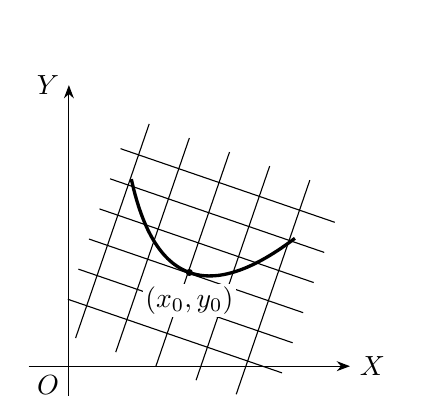
\begin{tikzpicture}[>=Stealth, scale=0.85]
  % Axes
  \draw[->] (-0.6,0) -- (4.2,0) node[right] {$X$};
  \draw[->] (0,-0.6) -- (0,4.2) node[left] {$Y$};
  \node[below left] at (0,0) {$O$};
  
  % Vertex
  \coordinate (V) at (1.8,1.4);
  
  % Family (一): Lines parallel to symmetry axis (direction approx (0.35, 1.0))
  \foreach \k in {-1.2, -0.6, 0.0, 0.6, 1.2} {
    \draw[thin] ({1.8 + \k - 0.5}, {1.4 - 0.35*\k - 1.4}) -- ({1.8 + \k + 0.6}, {1.4 - 0.35*\k + 1.8});
  }
  
  % Family (二): Lines perpendicular to symmetry axis (direction (1.0, -0.35))
  \foreach \h in {-0.9, -0.45, 0.0, 0.45, 0.9, 1.35} {
    \draw[thin] ({0.3 + 0.35*\h}, {1.9 + \h}) -- ({3.5 + 0.35*\h}, {0.8 + \h});
  }
  
  % Parabola opening along axis of symmetry (direction ~ 70 deg)
  % Local coords: u in [-1.3, 1.3], x = 1.8 + u*cos(-20) + 0.5*u^2*cos(70)
  % y = 1.4 + u*sin(-20) + 0.5*u^2*sin(70)
  \draw[very thick] plot[domain=-1.3:1.3, samples=60]
    ({1.8 + 0.94*\x + 0.35*0.6*\x*\x}, {1.4 - 0.34*\x + 0.94*0.6*\x*\x});
    
  % Vertex point
  \fill (V) circle (1.5pt) node[below=4pt, fill=white, inner sep=1pt] {$(x_0, y_0)$};
\end{tikzpicture}
\end{minipage}
\end{figure}

\begin{itemize}[leftmargin=2em]
  \item[（二）] 今取直線族
  \begin{equation}
  y = -\frac{1}{m}x+k \label{eq:b4s-a1-5}
  \end{equation}
  使與 \eqref{eq:b4s-a1-2} 中各直線垂直；則 \eqref{eq:b4s-a1-5} 切於拋物線 $f(x, y)=0$ 的充要條件是其切點正好是頂點 $(x_0, y_0)$。

  將 $y = -\frac{1}{m}x+k$ 代入 $f(x, y)=0$ 由判別式為 0 求出切點 $(x_0, y_0)$，換句話說，拋物線方程式 $f(x, y)=0$ 現在可以先作平移，
  \[
  \begin{cases}
  \bar{x} = x - x_0 \\
  \bar{y} = y - y_0
  \end{cases}
  \]
  使頂點 $=(0, 0)$ 為新座標的頂點。

  \item[（三）] 然後再用一般方法消去 $xy$ 項（轉軸或鏡射）。
\end{itemize}

\begin{example}
$\Gamma_0: 4x^2-4xy+y^2+8x+6y-7=0$

$\because \delta = -\begin{vmatrix} 4 & -2 \\ -2 & 1 \end{vmatrix} = 0, \quad \Delta \neq 0$ 故知為一拋物線。

設直線 $y=mx+b$ 平行於拋物線的對稱軸，則
\[
4x^2-4x(mx+b)+(mx+b)^2+8x+6(mx+b)-7=0
\]
中二次項係數應等於 0 即
\[
4-4m+m^2=0 \quad \therefore m=2.
\]
$\therefore$ 垂直於對稱軸的直線斜率為 $-\frac{1}{2}$。

設 $y=-\frac{1}{2}x+k$ 為過 $\Gamma_0$ 頂點的切線，則
\[
4x^2-4x\left(-\frac{1}{2}x+k\right)+\left(-\frac{1}{2}x+k\right)^2+8x+6\left(-\frac{1}{2}x+k\right)-7=0,
\]
即
\[
\frac{25}{4}x^2+(5-5k)x+(k^2+6k-7)=0 \quad (\text{有二重根}) \quad k=1.
\]
\begin{align*}
x &= \frac{-2(5-5k)}{25} = -\frac{2}{5}(1-k) = 0 \\
&\quad \bigl(\text{其中 } (5-5k)^2-25(k^2+6k-7)=0 \text{ 為判別式，解之得 } k=1\bigr).
\end{align*}
故
\[
\begin{cases}
x=0 \\
y=1
\end{cases}
\]
將座標軸中心平移至 $(0, 1)$ 點，即 $\bar{x}=x, \; \bar{y}=y-1$，得 $\Gamma_0$ 的方程式為
\[
4\bar{x}^2-4\bar{x}(\bar{y}+1)+(\bar{y}+1)^2+8\bar{x}+6(\bar{y}+1)-7=0
\]
$\therefore 4\bar{x}^2-4\bar{x}\bar{y}+\bar{y}^2+4\bar{x}+8\bar{y}=0$。

以下則利用固有值理論標準化：
\begin{itemize}[leftmargin=2em]
  \item[(i)] 消去 $xy$ 項：
  \[
  \begin{vmatrix}
  4-\lambda & -2 \\
  -2 & 1-\lambda
  \end{vmatrix} = \lambda^2-5\lambda \quad \therefore \lambda=0, \; \lambda=5.
  \]
  $\therefore$ 二次項標準化可得 $5{y'}^2$。

  \item[(ii)] 求轉軸後的基底向量：
  \[
  \begin{cases}
  (4-\lambda)\bar{x}-2\bar{y} = 0 \\
  -2\bar{x}+(1-\lambda)\bar{y} = 0
  \end{cases}
  \]
\end{itemize}

\begin{center}
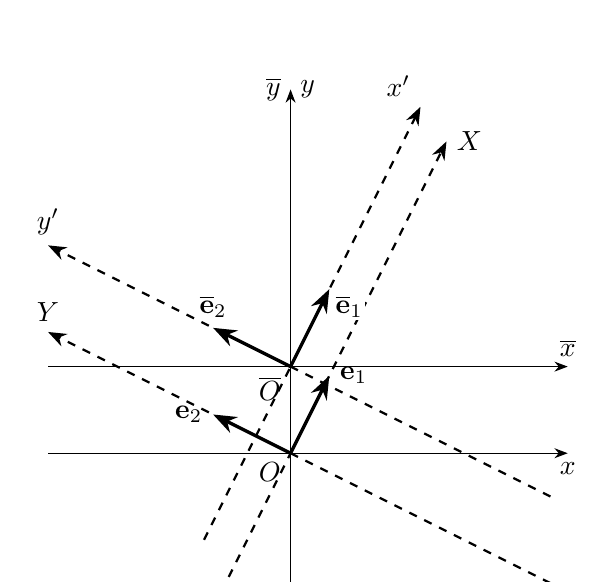
\begin{tikzpicture}[>=Stealth, scale=1.1]
  % Original horizontal axis at O(0,0)
  \draw[->] (-2.8,0) -- (3.2,0) node[below] {$x$};
  
  % Translated horizontal axis at \bar{O}(0,1)
  \draw[->] (-2.8,1) -- (3.2,1) node[above] {$\bar{x}$};
  
  % Vertical axis through O and \bar{O}
  \draw[->] (0,-1.5) -- (0,4.2);
  \node[left] at (0,4.2) {$\bar{y}$};
  \node[right] at (0,4.2) {$y$};
  
  \node[below left] at (0,0) {$O$};
  \node[below left] at (0,1) {$\bar{O}$};
  
  % Rotated axes through \bar{O}(0,1)
  % Slope 2: x'
  \draw[thick, dashed, ->] (-1.0,-1.0) -- (1.5,4.0) node[above left] {$x'$};
  % Slope -1/2: y'
  \draw[thick, dashed, ->] (3.0,-0.5) -- (-2.8,2.4) node[above] {$y'$};
  
  % Parallel dashed lines through O(0,0)
  % Slope 2: X
  \draw[thick, dashed, ->] (-0.8,-1.6) -- (1.8,3.6) node[right] {$X$};
  % Slope -1/2: Y
  \draw[thick, dashed, ->] (3.0,-1.5) -- (-2.8,1.4) node[above] {$Y$};
  
  % Basis vectors \bar{e}_1, \bar{e}_2 at \bar{O}
  \draw[->, very thick] (0,1) -- ({1/sqrt(5)}, {1 + 2/sqrt(5)}) node[below right=1pt, fill=white, inner sep=1pt] {$\bar{\mathbf{e}}_1$};
  \draw[->, very thick] (0,1) -- ({-2/sqrt(5)}, {1 + 1/sqrt(5)}) node[above=2pt, fill=white, inner sep=1pt] {$\bar{\mathbf{e}}_2$};
  
  % Basis vectors e_1, e_2 at O
  \draw[->, very thick] (0,0) -- ({1/sqrt(5)}, {2/sqrt(5)}) node[right] {$\mathbf{e}_1$};
  \draw[->, very thick] (0,0) -- ({-2/sqrt(5)}, {1/sqrt(5)}) node[left] {$\mathbf{e}_2$};
\end{tikzpicture}
\end{center}

取 $\lambda=0$ 得 $2\bar{x}=\bar{y}$。

取固有向量：$\bar{\mathbf{e}}_1 = \left(\frac{1}{\sqrt{5}}, \frac{2}{\sqrt{5}}\right)$。

再取 $\bar{\mathbf{e}}_2 = \left(-\frac{2}{\sqrt{5}}, \frac{1}{\sqrt{5}}\right)$\footnote{原書印為 $\bar{\mathbf{e}}_2 = \left(-\frac{1}{\sqrt{5}}, \frac{1}{\sqrt{5}}\right)$，第一分量分子誤植為 1，依正交單位向量與下文例 2 校訂為 $-\frac{2}{\sqrt{5}}$。}。

則新舊座標變換式為
\[
\begin{cases}
\bar{x} = \frac{1}{\sqrt{5}}x' - \frac{2}{\sqrt{5}}y' \\
\bar{y} = \frac{2}{\sqrt{5}}x' + \frac{1}{\sqrt{5}}y'
\end{cases}
\]
故得
\[
5{y'}^2+4\left(\frac{1}{\sqrt{5}}x'-\frac{2}{\sqrt{5}}y'\right)+8\left(\frac{2}{\sqrt{5}}x'+\frac{1}{\sqrt{5}}y'\right)=0,
\]
即
\[
5{y'}^2+4\sqrt{5}x'=0,
\]
\[
{y'}^2 = -\frac{4\sqrt{5}}{5}x'. \qquad \#
\]
\end{example}

\begin{example}
上例中的拋物線方程式，根據課文（$P_{229}$）先轉軸後平移的方法，解之如下以作為比較。

固定原點取
\[
\begin{cases}
\mathbf{e}_1 = \left(\frac{1}{\sqrt{5}}, \frac{2}{\sqrt{5}}\right) \\
\mathbf{e}_2 = \left(-\frac{2}{\sqrt{5}}, \frac{1}{\sqrt{5}}\right)
\end{cases}
\quad \text{則} \quad
\begin{cases}
x = \frac{1}{\sqrt{5}}X - \frac{2}{\sqrt{5}}Y \\
y = \frac{2}{\sqrt{5}}X + \frac{1}{\sqrt{5}}Y
\end{cases}
\]
則 $\Gamma_0$ 可化得：
\[
5Y^2-4\sqrt{5}X-2\sqrt{5}Y-7=0.
\]
由配方化簡得：
\[
\left(Y-\frac{1}{\sqrt{5}}\right)^2 = -\frac{4\sqrt{5}}{5}\left(X-\frac{2}{\sqrt{5}}\right).
\]
故所需平移為
\[
\begin{cases}
x' = X - \frac{2}{\sqrt{5}} \\
y' = Y - \frac{1}{\sqrt{5}}
\end{cases}
\]
即得
\[
{y'}^2 = -\frac{4\sqrt{5}}{5}x'.
\]
結果相同，注意 $\bar{O}=(0, 1)(O; x, y) = \left(\frac{2}{\sqrt{5}}, \frac{1}{\sqrt{5}}\right)(O; X, Y)$。\hfill $\#$
\end{example}

先轉軸再平移，不易見出新座標系原點相對於原座標系的座標，必須再經一次換算步驟。


\end{document}
